\section{Implementation}
In diesem Kapitel beschäftigen wir uns mit der Implementation und mit dem Aufbau von Grafana, sodass wir \gls{Cyberangriff} nach dem \gls{mitre} Matrix erkennen können. Wir gestalten unser Arbeitslabor mit \gls{container} und \glsfirst{vm}, wie in dem folgenden Diagramm:

\begin{figure}[H]
   \centering
   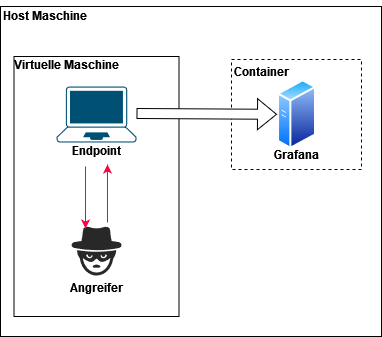
\includegraphics[width=0.6\textwidth]{assets/Arbeitslabor.drawio.png}
   \caption{Aufbau unseres Arbeitslabors \\Quelle: Eigene Quelle}
   \centering
\end{figure}

Von unserem Aufbau zielen wir, die Aufnahmen und Anpassung der Logdateien für Grafana, die Musterkerennung für die ausgewählten \glsplural{Cyberangriff} und schließlich die Warnmeldung für die Endnutzer, sodass sie sich für entsprechende Sicherheitsmßnahmen entscheiden können. Dieser Ablauf ist in dem folgenden Diagramm dargestellt:

\begin{figure}[H]
   \centering
   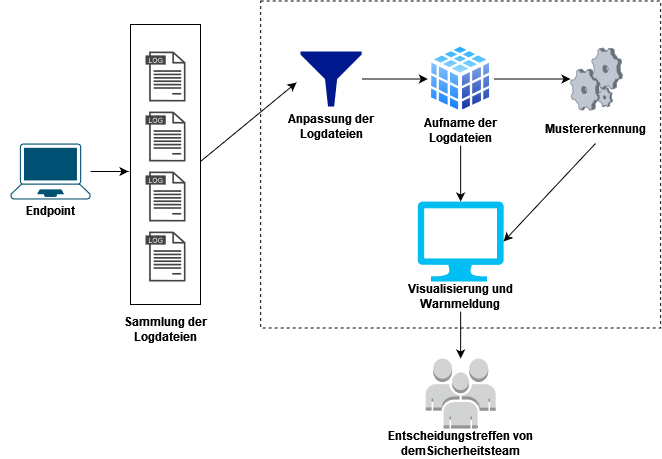
\includegraphics[width=0.8\textwidth]{assets/Ablauf_grafana.drawio.png}
   \caption{Erwarteter Ablauf von der Datensammlung bis zur Warnmeldung von \glsplural{Cyberangriff} \\Quelle: Eigene Quelle}
   \centering
\end{figure}

\subsection{Angriffserkennung mithilfe von Mitre ATT\&CK Matrix\textregistered}
Es gibt verschiedene Methode und Framework zur Vermeidung, Erkennung, und Unterbrechung von \glsplural{Cyberangriff}. \glsfirst{owasp}, \glsfirst{CKC} und \gls{mitre} Matrix sind einige Bespiele von denen, die \gls{SOC}-Teams verwenden, um Sicherheit von Systemen und/oder Netwerken zu gewährleisten. Da die Richtlinien und Fokus von diesen Frameworks sich unterscheiden können und deswegen anderen Aufbau von unserer Struktur verlangen wurden, entschieden wir uns für die Anwendung von der \gls{mitre} Matrix für die Erkennung der \glsplural{Cyberangriff} besonders, weil dieser Framework auch an Splunk integriert ist.

\newpage
Die \gls{mitre} Matrix hat folgende Hauptnutzung \citep{Mitre_Started}:

\begin{itemize}[noitemsep]
   \item Erkennung und Analyse von Angriffstechnik
   \item	strukturierte Datensammlung über Bedrohungen
   \item	Emulieren von \glsplural{Cyberangriff} für die Anwendung an Angriffsübungen
   \item	Systemhärtung und Verbesserung der Verteidigungsmaßnahmen
\end{itemize}

Die Matrix bietet eine umfangreiche Verwendung für Unternehmen und für \gls{SOC}-Team an, um ihre wertvollen Resource schützen und ihre Fachkenntnisse über \gls{Cybersicherheit} zu erweitern \citep{Hazel_howtousemitre}. Hier konzentrieren wir uns auf die Entwicklung und auf die Implementierung einer Methode für die automatische Erkennung und Analyse von Angriffstechnique in Grafana.

Die \gls{mitre} Framework besteht aus 14 Taktik. Zu jedem Taktik gehören Technique, die ihrerseits in Subtechniques aufgeteilt sind. Jede Subtechnique wird mit Beispielen, Härtungsmaßnahmen und Erkennungsregeln dargestellt. Die Folgebende Abbildung zeigt, wie diese Struktur aufgebaut ist: 

\begin{figure}[H]
   \centering
   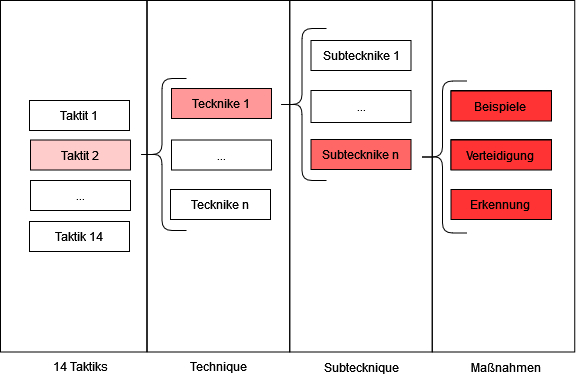
\includegraphics[width=0.8\textwidth]{assets/Mitre_structure.drawio.png}
   \caption{Struktur der Mitre Matrix \glsplural{Cyberangriff} \\Quelle: Eigene Quelle}
   \centering
\end{figure}

\newpage
Die 14 Tactics sind folgende:
\begin{itemize}[noitemsep]
   \item Informationssammlung für zukünftige Angriffe 
   \item	Entwicklung von Ressource von Angreifer
   \item Erster Zugang zum Opfersysteme 
   \item Ausführung von bösartigen Coden
   \item Beharrlichkeit von System
   \item	Privilegienausweitung
   \item Vermeidung von Verteidigungssysteme
   \item Zugang zu Anmeldedaten
   \item Umgebungserkennung
   \item Seitliche Bewegung zu anderem Systemen innerhalb des Angriffsziels
   \item internet Informationssammlung
   \item Steuerung und Kontrolle (C2 - Command and Control im Original)
   \item Datenextrahierung 
   \item	Auswirkung auf die Integrität
\end{itemize}

In dieser Arbeit beschäftigen wir uns mit Tactic "Zugang zu Anmeldedaten" und deren Technique \gls{bruteforce}. Diese Technique ist in vier Subtechnique aufteilt
\begin{itemize}[noitemsep]
   \item Erraten von Anmeldedaten 
   \item	Entschlüsselung von \glsplural{hash}
   \item \textit{\gls{spraying}}
   \item \textit{\gls{stuffing}}
\end{itemize}

Um den Umfang dieser Arbeit an ihren Einschränkungen anzupassen, lassen wir unseren Fokus auf die Erkennung der Subtechnique Erraten von Anmeldedaten und \textit{\gls{stuffing}}, da diese Angriffe ähnliche Erkennungmethode haben. Hier schließen wir auch die anderen Maßnahmen aus.

\newpage
Die nächste Abbildung zeigt den Umfang unseres Implementationsversuchs:

\begin{figure}[H]
   \centering
   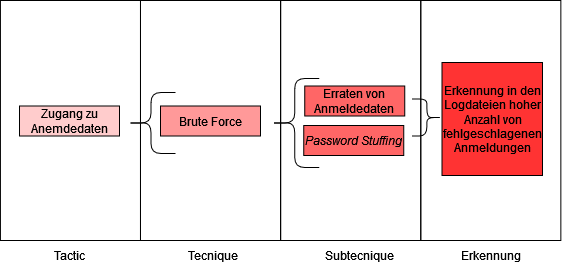
\includegraphics[width=0.8\textwidth]{assets/T1110.drawio.png}
   \caption{Analysestruktur für diese Arbeit \glsplural{Cyberangriff} \\Quelle: Eigene Quelle und \citep{Mitre_t1110}}
   \centering
\end{figure}

\subsection{Aufbau der Erkennungsregel für den ausgewählten Angriff}
Der \gls{bruteforce} lässt sich durch die Anzahl des fehlgeschlagen Anmeldungsversuchs erkennen \citep{Selvaganesh_SplunkBruteForce}. Wir bearbeiten eine Situation, in der es keine Gegenmaßnahmen, wie Kontosperre nach \textit{n} beliebigen Versuchen oder \gls{mfa}, implementiert sind. Das folgende Aktivitätsdiagramm stellt einen allgemeinen Ablauf eines Anmeldungsverfahrens dar:

\begin{figure}[H]
   \centering
   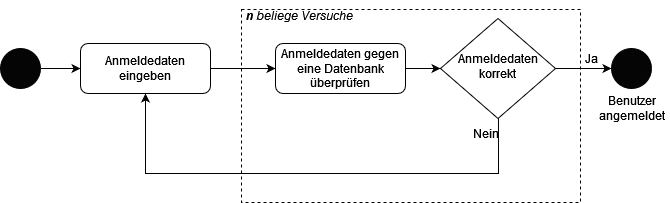
\includegraphics[width=0.8\textwidth]{assets/Anmeldeverfahren.drawio.png}
   \caption{Allgemeiner Ablauf eines Anmeldungsverfahrens \\Quelle: Eigene Quelle und \citep{Selvaganesh_SplunkBruteForce}}
   \centering
\end{figure}

\textcolor{red}{\textbf{Regel von SPLUNK hinzufügen, wie sollten unsere Regel aussehen=}}
\textcolor{red}{\textbf{statische vs dinymische Regel}}




\subsection{Bewertung der Daten in Grafana}
Hinzufügen der Logdateien und Erstellung von Regeln zur Erkennung des Angriffes
Diagramm der Nutzung von Grafana

\subsection{Normalisierung der Logdateien mit Zeek}
Diagramm der Nutzung von Grafana und Zeek

Hier werden die Schritte für die Installation und Sammeln von Daten beschrieben.

- Implementation in Container %https://rdr-it.com/elk-installation-configuration-un-siem-docker/


\subsection{Sammlung von Server-Log Dateien}

\subsection{Normalisierung der Log-Dateien}





